\documentclass[10pt,conference]{IEEEtran}
\usepackage{cite}
\usepackage{amsmath}
\usepackage[T1]{fontenc}
\usepackage{graphicx}
\usepackage{url}
\usepackage{hyperref}
\usepackage{booktabs}
\usepackage{tabularx}
\usepackage{array}
\begin{document}
\title{Auditing Artificial Intelligence Benchmarks with Coding Agents}
\author{Anonymous authors}
\maketitle
\begin{abstract}
\textbf{Background:} Reviewing an artificial intelligence benchmark means asking separate questions about its evaluation software, its documentation and the interpretation attached to its scores. Existing checklists and measurement guidance tell a reviewer what to look for, but they do not record what evidence the reviewer had, and they do not separate missing information from demonstrated defects.
\textbf{Objective:} We introduce MESA, a benchmark audit rubric with ten criteria and evidence states, and examine how coding agents apply it when they can read only the paper and README (Input 1) and when they can also list and read the text files of a fixed repository snapshot (Input 2).
\textbf{Method:} Two sequential batches, GPT-6 Luna through Codex and Claude Fable 5.1 through Claude Code, each reviewed HumanEval, TruthfulQA and DesignQA under both inputs with two repetitions, giving 12 sessions and 120 judgments per batch. Prompts, sources, reference proposals and the analysis plan were fixed before each batch. Analysis is offline and reproducible from the saved responses.
\textbf{Results:} All 24 sessions returned structurally valid responses. Repository access changed judgments mainly on the software criteria, and in the Claude batch only on them. Repeated sessions agreed on 46 of 60 and 55 of 60 judgments; the two batches agreed on 92 of 120. Repository sessions surfaced code and documentation discrepancies the papers do not mention, and some ratings exceeded the support stated in their own reasons.
\textbf{Conclusion:} The rubric and procedure make the evidence behind each judgment inspectable. Repository access changes what an agent can inspect without settling what the evidence means, so the division of review work between agents and people remains a design question. The study does not establish rubric validity, human usability or benchmark quality.
\end{abstract}
\begin{IEEEkeywords}
benchmark review, measurement, coding agents, evidence, software evaluation, human and AI collaboration
\end{IEEEkeywords}

\section{Introduction}
Benchmark review is work that people do. Program committees, leaderboard maintainers, procurement teams and researchers who adopt a benchmark all have to decide whether its scores support the claims attached to them. The decision rests on three different kinds of evidence. An evaluation script can implement its stated formula and still produce a score that does not support the intended claim. Missing documentation does not establish that a benchmark was built incorrectly. A documented checking procedure does not imply that its findings were favorable. Test review and score validation guidance from psychological measurement separates these questions \cite{efpa_test_review_model_2025,kane_validation,aera_apa_ncme_standards_2014}, and benchmark research has shown how often they are blurred in practice \cite{reuel_betterbench,bean_measuring_what_matters,jo_wilson_what_does_your_benchmark_measure}.

Coding agents are now proposed as collaborators in this work. They can list files, read source, compare a definition with an implementation and locate documentation. Whether that help changes a review, and which parts of the review stay with the person, is an open question. In this study the agents receive a confined file listing and text reader over a fixed snapshot; they do not run tests, browse or inspect images, so our results concern this restricted form of inspection rather than an unrestricted repository audit.

We develop MESA as a benchmark audit rubric with ten criteria. This is a research revision of the project, distinct from its earlier questionnaire with 25 questions. Each criterion has anchors that name the evidence a rating requires, and two null states, insufficient evidence and not applicable, keep missing information apart from defects. We then ask:

\begin{itemize}
\item \textbf{RQ1.} What evidence do coding agents record when applying the criteria, and does the recorded evidence support the ratings they assign?
\item \textbf{RQ2.} How do judgments change when repository text files become available alongside the paper and README?
\item \textbf{RQ3.} How much do judgments vary between two repetitions of the same configuration, and how much do two configurations agree?
\end{itemize}

The questions do not assume that repository access improves judgments or that software inspection settles measurement questions. Our contributions are: (1) the rubric, with its design decisions and omissions stated; (2) a procedure for collecting agent review evidence under fixed inputs, without exposing reference judgments, with every citation checkable afterwards; (3) observations from two sequential batches on three benchmarks, including repository discrepancies that neither paper reports; and (4) a replication package with raw responses, event logs and offline analysis. Human evaluation of the rubric is future work and is not a prerequisite for the model study.

Throughout, a \emph{session} is one agent review of one benchmark under one input; a \emph{batch} is the twelve sessions run with one configuration; a \emph{judgment} is a status plus, when rated, a \emph{rating} for one criterion.

\section{Background and Related Work}
\subsection{Test review and score validity}
The European Federation of Psychologists' Associations Test Review Model separates describing a test from evaluating its properties and its use; its 2025 edition runs to 90 pages of forms and guidance \cite{efpa_test_review_model_2025}. Validity, in this tradition, is a property of an interpretation and use of scores, not of a test in isolation \cite{kane_validation,aera_apa_ncme_standards_2014}. A benchmark intended to compare performance on a stated set of tasks need not establish performance on a wider domain, and a human parity claim creates a different evidence requirement from a comparison among models. MESA inherits the distinction between identifying a scoring rule, checking its implementation and finding favorable results, and allows inapplicability with a reason when a criterion does not arise for the stated use.

Cohn and Hernández-Orallo bring this tradition to AI evaluation instruments, their umbrella term for benchmarks, competitions and datasets \cite{cohn_hernandez_orallo_oecd_2023}. Their framework characterises an instrument with eighteen facets grouped under validity, consistency and fairness, each taking categorical values. Some facets classify rather than evaluate: Judgeability records whether scoring is manual, automated or mixed, and Reference records whether scores are reported as absolute values or relative to a norm such as human performance. Others carry a preferred value, such as Reliability in the test-retest sense. The authors report that their raters needed literature beyond an instrument's own specification to judge Coverage and Specificity, and that those facets, with Capability, Adjustability and Ambition, produced the least agreement. That observation motivates our second input: a specification alone does not settle these judgments, so we test what repository access adds.

The two frameworks are complementary rather than competing. A facet value describes what kind of instrument a benchmark is; a MESA judgment audits the evidence the sources give about it. Three pairs share ground and answer different questions. The Reliability facet says whether an instrument is reliable; MESA's B3 says what evidence the sources give about variation. The Reference facet says whether a human norm is used; B4 asks whether the human procedure supports the comparison. Judgeability says who scores; A2 asks whether automated scoring matches its documented rule, and applies only when Judgeability is automated or mixed. Three words need care. The framework's ``contaminated'' means results contaminated by other skills or tasks, not training data, so MESA's B5 is named training exposure. Its ``reproducibility'' means that the same test can be generated again, whereas A5 concerns instructions a reader can follow. Its ``static'' is a value of the Progression facet, so we call our snapshots fixed, the framework's own term for an unchanging dataset.

\subsection{Benchmark quality and documentation}
BetterBench assesses benchmark design, implementation, documentation and maintenance through 46 criteria and the numerical labels 0, 5, 10 and 15 \cite{reuel_betterbench}. It motivates attention to evaluation code, data descriptions, dependencies and reproduction instructions. Documentation standards for datasets and models name the fields a reviewer should expect to find \cite{gebru_datasheets_2021,mitchell_model_cards_2019}. Evidence centred benchmark design asks that a benchmark state what it measures and why its tasks are evidence for that claim \cite{liu_ecbd_2024}. Studies of benchmark practice report that many benchmarks do not state the ability they claim to measure, do not justify task selection, do not report uncertainty, and that leaderboard procedures can distort comparisons \cite{bean_measuring_what_matters,jo_wilson_what_does_your_benchmark_measure,cheng_benchmarking_broken,singh_leaderboard_illusion}.

These sources tell a reviewer what to look for. They do not record what evidence the reviewer actually had, whether a repository was inspected, or how a missing statement should be distinguished from a demonstrated defect. An aggregate score lets both produce the same number. The existence of a script does not show that it executes; reading code supports a comparison with a formula but is not an execution test; a README may describe reproduction without anyone having reproduced. MESA keeps these differences in the evidence record and reports no total score.

\subsection{Language models as evaluators}
Work on language models as judges shows that repeated judgments vary and that presentation affects outcomes \cite{zheng_llm_judge_2023,shi_judging_judges_2025}. That work grades generated answers. Auditing a benchmark is a different task: the agent examines evidence about software and documentation, not a single response, and the object of interest is the evidence record it produces. We therefore adopt the repeat and compare discipline of that literature while reporting observations about applying a rubric rather than certifying a benchmark.

\section{The MESA Audit Rubric}
Table~\ref{tab:criteria} states the ten criteria. Every response contains, for each criterion, a status, a rating when supported, a reason, evidence locators with short quotes, missing information and checks performed, plus a limits statement for the session. Ratings concern each criterion's defined requirement and are never added or averaged.

\begin{table*}[t]
\caption{The ten audit criteria and the evidence each seeks.}
\label{tab:criteria}
\small
\begin{tabularx}{\textwidth}{@{}lp{0.19\textwidth}X@{}}
\toprule
ID & Criterion & Evidence sought \\
\midrule
A1 & Evaluation scripts & An evaluation entry point, inspectable implementation and evidence of execution for the relevant edition. \\
A2 & Scoring implementation & A comparison of the implemented rule with its description, and checks of behavior and relevant edge cases; applies when scoring is automated or mixed. \\
A3 & Dataset documentation & Instance format, partitions, provenance and relevant metadata. \\
A4 & Permissions and dependencies & Reuse terms for the supplied data and code, plus software requirements and version constraints. \\
A5 & Reproduction instructions & Steps for obtaining data, setup, execution and interpretation of output; not demonstrated reproduction. \\
B1 & Construct definition & The target ability, its operational definition and the limits of interpretation. \\
B2 & Answer checking & Checking procedures for tasks and reference answers, their coverage, findings and limits. \\
B3 & Score reliability & Variation and uncertainty, in the test-retest sense, relevant to the intended comparison. \\
B4 & Human comparisons & Sampling, tasks, conditions and scoring when a norm-referenced human comparison supports a claim. \\
B5 & Training exposure & Assessment of prior exposure to test tasks or answers, safeguards, checks and remaining limits. \\
\bottomrule
\end{tabularx}
\end{table*}

\subsection{Design decisions}
The ten criteria are a research design decision, not a validated reduction of the earlier questionnaire. We chose concerns a reviewer can address from a paper and a repository snapshot: five that repository text can inform directly, and five measurement concerns that benchmark papers commonly address and that the measurement literature treats as separate questions. Each criterion receives one judgment so that evidence, missing information and checks stay attached to a single requirement.

We retained the labels 0, 5, 10 and 15 from BetterBench because benchmark authors know them, but labels alone do not define requirements. Each criterion therefore has anchors that distinguish a claim, an inspectable artifact and a documented check. For A1, a claim that code exists supports 5, an inspectable implementation without established execution supports 10, and implementation with documented execution for the edition supports 15. For A5, the highest anchor concerns complete instructions, not demonstrated reproduction. For B2, documented checking may reach 15 even when errors were found, provided procedure, coverage, findings and limits are stated. When no anchor is supported the status is \emph{insufficient evidence} with a null rating; \emph{not applicable} also has a null rating and requires a reason tied to the intended claim. In the terms of the facet framework, A2 is expected to be not applicable when Judgeability is manual, and B4 when Reference is absolute.

We considered and set aside three alternatives: keeping the 25 question instrument with repository inspection, which would have left most questions without a repository check; an aggregated benchmark score, which hides the difference between documentation and evidence requirements; and execution based checks, which need sandboxing and resource decisions outside this scope. A correspondence map between the ten criteria and the earlier questions is kept with the study materials as a conceptual map, not a derivation. None of these decisions has been validated by content review or human use.

\subsection{Relation to the earlier questionnaire and to the facet framework}
The earlier questionnaire covered description, development, scoring, consistency, meaning, fairness and use through 25 questions. The ten criteria combine some concerns and omit others: score aggregation, shortcuts unrelated to prior exposure, training and submission rules, comparisons across systems, release changes and the scope of public claims are not separately preserved. Against the facet framework, MESA has no counterpart for Coverage and Capability as representativeness judgments, nor for Realism, Purpose, Ambition, Adjustability, Containedness, Partiality, Autonomy, Antecedents or Progression. B1 asks for the ability and its operationalization but not whether the task set is representative; the framework's raters found exactly that judgment hard to make from specifications. The rubric is therefore a selected audit, not a complete test review model or construct validity assessment. The software and measurement groups organize reporting; they are not two validated scales.

\section{Study Design}
Figure~\ref{fig:method} summarizes the procedure. Fixed sources form two inputs: Input 1 holds the paper text and README; Input 2 adds a file listing and text reader over the repository snapshot. Each session applies the rubric and returns a structured response. All analysis is performed offline on the saved responses. We followed the empirical standards recommended by the venue where they apply to a repeated measurement study without human participants \cite{sigsoft_empirical_standards}.

\begin{figure*}[t]
\centering
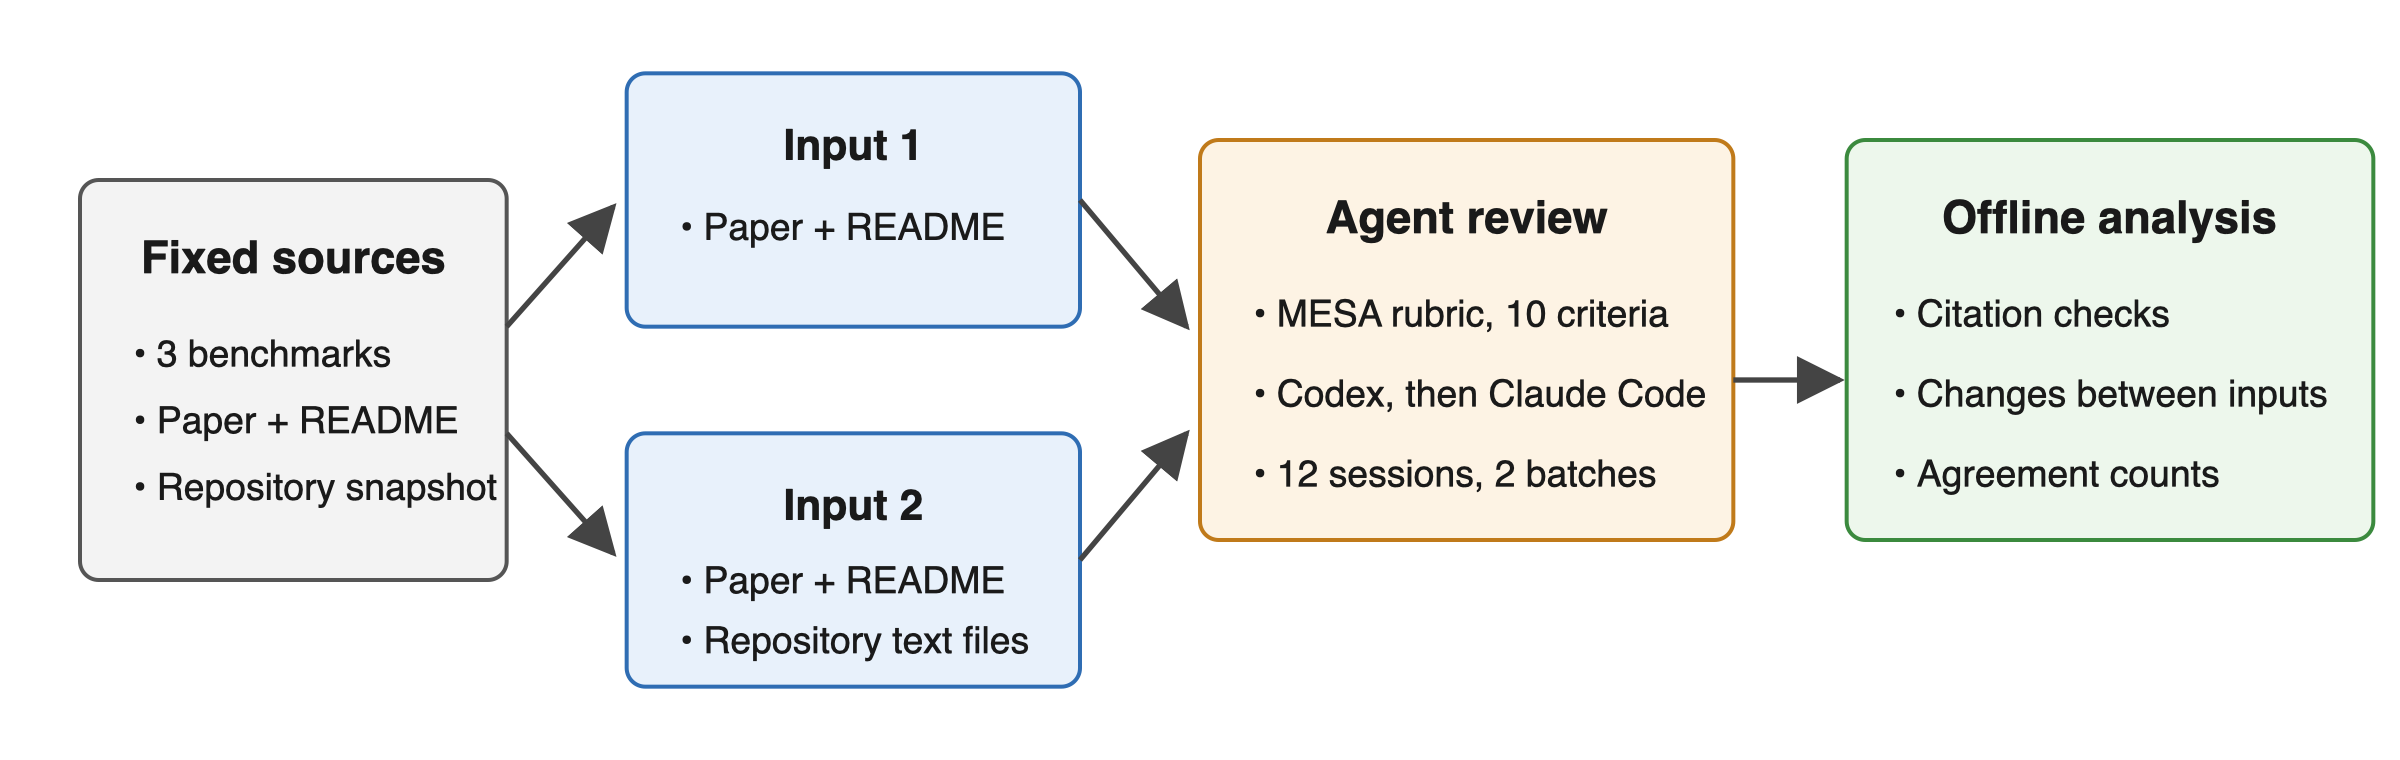
\includegraphics[width=0.92\textwidth]{figures/v3_method_diagram.png}
\caption{Study procedure. Fixed paper text, README and repository snapshot form two inputs: Input 1 holds the paper and README, Input 2 adds the repository text files. Each session applies the ten criterion rubric in one of two sequential batches and returns a structured response. Counts, citation checks and the selected audit are computed afterwards from saved responses.}
\label{fig:method}
\end{figure*}

\subsection{Benchmarks and sources}
We selected HumanEval, TruthfulQA and DesignQA to cover programming tasks, truthfulness questions and engineering documentation \cite{human_eval_repository,truthfulqa_repository,doris_designqa_2024}. The selection reflects scope and resource constraints, not a representative sample. Each benchmark has a fixed repository commit, a retrieved paper PDF and extracted text; a source manifest records retrieval times, hashes and file inventories. The paper and repository need not describe the same edition: HumanEval's README marks the repository as unmaintained, and TruthfulQA's README describes a 2025 multiple choice revision beyond the original tasks. Such differences are evidence to report, not to reconcile. The review concerns the interpretation stated in the paper, bounded by its reported tasks.

Both inputs contain the complete extracted paper text and the top level README. Input 2 additionally exposes file listing and text reading for the snapshot. It cannot execute code, write files, browse or inspect other study files. Binary files, including DesignQA's images, are retained but unreadable through the text reader. Paper extraction can lose layout and figure content.

\subsection{Inputs and reviewer configurations}
The first batch used GPT-6 Luna at medium reasoning effort through Codex \cite{openai_codex_execution}; the second, run after the first had completed, used Claude Fable 5.1 at medium reasoning effort through Claude Code \cite{anthropic_claude_code_cli}. In each batch, three benchmarks, two inputs and two repetitions yield twelve main sessions, with two pilot sessions on a fictional fixture. Each batch had an attempt cap of sixteen, including pilots and permitted infrastructure retries, and no per session token, output, tool call or time ceilings beyond account limits.

Every session started in an empty temporary directory. The Codex runner disabled inherited project instructions, host skills, memory, shell, image, browser, plugin and multi agent features. The Claude Code runner replaced the default system prompt with the study instruction, loaded no user or project settings, disabled skills and every built in tool, accepted only the command line supplied tool server, denied any permission prompt and requested structured output against the response schema. Input 2 sessions received only a file server confined to the snapshot, with path checks against traversal and symlink escapes. Source content was treated as data, not instructions. Both inputs and both batches used the same rubric, fictional teaching example, prompts and response schema; the prompt files are byte identical across batches.

Every session applied the rubric. There is no session without it and none with another instrument, so the study examines how agents apply MESA under two inputs and two configurations; it cannot show that MESA improves reviews relative to unstructured review. Order was randomized within repetition blocks with a recorded seed per batch, and sessions ran sequentially. The input contrast estimates the effect of adding repository evidence and a means to inspect it together; it does not separate a tool effect from an information effect. The two batches differ in provider, model, command line tool and harness at once and were not jointly randomized, so their comparison is descriptive agreement between two configurations, not a model or tool effect.

\subsection{Procedure and pilots}
Both Codex pilots produced structurally valid responses. The Input 2 pilot's file listing was refused because the tool required approval; it was retained as an input delivery failure, the runner was changed to approve the two read only tools automatically, and an ignored image tool setting was corrected before the materials were fixed. Offline fixture checks verified permitted reads, rejection of paths outside the snapshot and response validation. The rubric was not changed in response to pilot judgments.

The Claude batch had its own pilots and freeze. Its first Input 1 pilot attempt failed before any model request because Claude Code rejected the schema declaration key in the fixed response schema; the runner was changed to omit only that key from the command line argument, the schema file and validation rules are unchanged, and the failed attempt is retained. The second Input 1 pilot and the Input 2 pilot then completed, and the Input 2 pilot read files under the tool names Claude Code assigns although the prompt names them in the Codex form, so the prompts were left unchanged. Claude Code also made an auxiliary call to a smaller model in every session; its inputs are not exposed in the event records, and the review content comes from messages attributed to the requested model.

\subsection{Analysis}
Sixty assistant reference proposals, one per benchmark, criterion and input, were prepared before the first batch and not changed for the second. None was independently checked; all are provisional or contested, and they are not an expert baseline. We therefore report no accuracy against experts and treat agreement with a proposal as agreement, not correctness.

The offline analysis validates response structure, resolves cited sources within the allowed set, checks exact and whitespace normalized quote matches separately, and checks whether a parseable locator resolves. These mechanical checks are separate from whether an excerpt supports a rating, and a failed match can reflect paraphrase, ellipsis or extraction rather than fabrication. Repeat agreement requires the same status and rating in both repetitions; input comparisons pair Input 1 and Input 2 within benchmark and repetition; batch comparisons pair the two batches within benchmark, input and repetition. Only structurally usable responses with delivered inputs enter comparisons, and all denominators remain visible. No significance test treats the judgments as independent. A selected audit covers repetition one for every benchmark and input in each batch, sixty judgments per batch, without substituting cases. For each repository discrepancy reported by an agent, the preparing assistant later read the cited lines offline and recorded scope and consequence; nothing was executed.

\section{Results}
Table~\ref{tab:execution} gives the execution accounting and mechanical checks for both batches. Tables~\ref{tab:ratings-codex} and~\ref{tab:ratings-claude} show where the judgments fell for each criterion and input.
\begin{table}[t]
\caption{Execution accounting for both batches.}
\label{tab:execution}
\centering\begin{tabular}{lrr}\toprule
Measure & Codex & Claude \\
\midrule
Planned main sessions & 12 & 12 \\
Attempted main sessions & 12 & 12 \\
Completed main responses & 12 & 12 \\
Structurally usable responses & 12 & 12 \\
Input delivered & 12 & 12 \\
Main criterion judgments & 120 & 120 \\
Pilot attempts & 2 & 3 \\
All physical attempts & 14 & 15 \\
Repeat pairs matching & 46 & 55 \\
Input pairs matching & 42 & 45 \\
Evidence citations & 295 & 460 \\
Citations to allowed existing sources & 295 & 459 \\
Exact quote matches & 122 & 299 \\
Whitespace normalized quote matches & 189 & 356 \\
Locators that resolve & 205 & 315 \\
\bottomrule\end{tabular}
\end{table}

\begin{table}[t]
\caption{Codex batch: judgments per criterion and input over six usable responses per input (IE: insufficient evidence; NA: not applicable).}
\label{tab:ratings-codex}
\centering\small\begin{tabular}{llrrrrrr}\toprule
Criterion & Input & 0 & 5 & 10 & 15 & IE & NA \\
\midrule
A1 & 1 & 0 & 2 & 4 & 0 & 0 & 0 \\
 & 2 & 0 & 0 & 6 & 0 & 0 & 0 \\
A2 & 1 & 0 & 2 & 4 & 0 & 0 & 0 \\
 & 2 & 0 & 0 & 6 & 0 & 0 & 0 \\
A3 & 1 & 0 & 0 & 4 & 2 & 0 & 0 \\
 & 2 & 0 & 0 & 5 & 1 & 0 & 0 \\
A4 & 1 & 0 & 1 & 5 & 0 & 0 & 0 \\
 & 2 & 0 & 0 & 5 & 1 & 0 & 0 \\
A5 & 1 & 0 & 0 & 4 & 2 & 0 & 0 \\
 & 2 & 0 & 0 & 3 & 3 & 0 & 0 \\
B1 & 1 & 0 & 0 & 0 & 6 & 0 & 0 \\
 & 2 & 0 & 0 & 0 & 6 & 0 & 0 \\
B2 & 1 & 0 & 0 & 4 & 2 & 0 & 0 \\
 & 2 & 0 & 0 & 3 & 2 & 1 & 0 \\
B3 & 1 & 0 & 0 & 6 & 0 & 0 & 0 \\
 & 2 & 0 & 0 & 6 & 0 & 0 & 0 \\
B4 & 1 & 0 & 0 & 3 & 0 & 0 & 3 \\
 & 2 & 0 & 1 & 2 & 0 & 0 & 3 \\
B5 & 1 & 0 & 1 & 5 & 0 & 0 & 0 \\
 & 2 & 0 & 2 & 4 & 0 & 0 & 0 \\
\bottomrule\end{tabular}
\end{table}

\begin{table}[t]
\caption{Claude batch: judgments per criterion and input over six usable responses per input (IE: insufficient evidence; NA: not applicable).}
\label{tab:ratings-claude}
\centering\small\begin{tabular}{llrrrrrr}\toprule
Criterion & Input & 0 & 5 & 10 & 15 & IE & NA \\
\midrule
A1 & 1 & 0 & 5 & 1 & 0 & 0 & 0 \\
 & 2 & 0 & 0 & 6 & 0 & 0 & 0 \\
A2 & 1 & 0 & 4 & 2 & 0 & 0 & 0 \\
 & 2 & 0 & 0 & 6 & 0 & 0 & 0 \\
A3 & 1 & 0 & 0 & 4 & 2 & 0 & 0 \\
 & 2 & 0 & 0 & 3 & 3 & 0 & 0 \\
A4 & 1 & 0 & 0 & 6 & 0 & 0 & 0 \\
 & 2 & 0 & 0 & 4 & 2 & 0 & 0 \\
A5 & 1 & 0 & 0 & 2 & 4 & 0 & 0 \\
 & 2 & 0 & 0 & 1 & 5 & 0 & 0 \\
B1 & 1 & 0 & 0 & 0 & 6 & 0 & 0 \\
 & 2 & 0 & 0 & 0 & 6 & 0 & 0 \\
B2 & 1 & 0 & 2 & 2 & 2 & 0 & 0 \\
 & 2 & 0 & 2 & 2 & 2 & 0 & 0 \\
B3 & 1 & 0 & 0 & 6 & 0 & 0 & 0 \\
 & 2 & 0 & 0 & 6 & 0 & 0 & 0 \\
B4 & 1 & 0 & 2 & 2 & 0 & 0 & 2 \\
 & 2 & 0 & 2 & 2 & 0 & 0 & 2 \\
B5 & 1 & 0 & 0 & 6 & 0 & 0 & 0 \\
 & 2 & 0 & 0 & 6 & 0 & 0 & 0 \\
\bottomrule\end{tabular}
\end{table}


\subsection{RQ1: Evidence recorded and its support for ratings}
Every citation in both batches but one resolved to an allowed source file; the exception cites the file listing itself. Exact quote matches were found for fewer than half of Codex citations and about two thirds of Claude citations, with whitespace normalization raising both. Beyond the mechanical checks, the selected audits show ratings that exceed the support stated in their own reasons, and repository sessions recorded discrepancies between code and documentation that neither paper reports.
\subsubsection{Reading a file and supporting a rating}
The selected DesignQA Input 2 response assigns A2 a rating of 10 while stating that no inspected code to rule comparison was established. That comparison is required by the anchor. The event record shows that the metric file was read, but the response does not explain the comparison needed to support the rating. One evidence entry describes the file as present rather than quoting its contents. File access and file existence therefore do not suffice to establish support for the judgment.

The selected HumanEval and TruthfulQA Input 1 responses give A1 a rating of 10 despite receiving no repository implementation. Their cited README commands identify entry points without exposing those implementations. The corresponding Input 2 responses also use 10, with code inspection available. Equal ratings can thus hide different evidence and different adherence to an anchor.

\subsubsection{Repository findings that the paper does not contain}
Several Input 2 responses record observations from inspection rather than from the paper. The preparing assistant later read the cited lines offline and assessed their scope; that review is retained with the analysis and has not been checked by a human author. For HumanEval, the response reports that the README describes the execution call as commented out while the shipped file has it active, and that a README file name does not exist in the snapshot. Both are confirmed in the snapshot; the consequence is a mismatch between the safety notice and the shipped harness, not a scoring difference. For TruthfulQA, the response reports an undocumented fixed reference answer appended to the true answer list before similarity scoring. The code does this for every reference comparison metric on generated answers; the paper defines non-committal answers as true, so the step implements the stated definition, and what is missing is documentation of the implementation rather than a rule violation. For DesignQA, the response reports that the similarity metric in the paper is commented out in the shipped code, so one column of the paper's results table cannot be regenerated from this snapshot, and that the overall score divides by a fixed six. The divisor only misstates the overall score when fewer than six subsets are supplied, which the README does not describe as a supported use.

None of these findings was established through execution, and none shows that a reported score is wrong. They show what a text reader over a snapshot can surface that the paper does not state. The responses rate A2 as 10 rather than 0 in these cases, arguing that the main documented rule is matched. Whether a commented out metric that appears in a results table is a rule violation under anchor 0 is a judgment the rubric wording leaves open; recording the discrepancy and judging its consequence for the reported results are different steps, and only the first occurred in the sessions.


\subsection{RQ2: Changes between inputs}
Repository access changed 18 of 60 paired judgments in the Codex batch, 14 of them on software criteria, and 15 of 60 in the Claude batch, all on software criteria. No measurement judgment changed with input in the Claude batch. Several changes concern sufficiency thresholds applied to text present in both inputs rather than facts available only in the repository.
\subsubsection{Scope and sufficiency}
The selected HumanEval Input 1 response gives B2 a rating of 10 while saying that a checking procedure for HumanEval answers is not reported. It cites verification for a separate training set. The Input 2 response instead uses insufficient evidence. This is an example of why an excerpt must concern the benchmark and check being judged; locating the words in the paper is not enough.

For HumanEval B4, the Input 1 response uses not applicable, while the Input 2 response uses 5 because the paper discusses expected student performance. Both received the same paper. The difference concerns whether the review includes that wider comparison or only measured benchmark results. The present reference proposal does not independently settle that scope choice.

Other changes also concern thresholds applied to shared text. For DesignQA A5, the Input 2 response lowers the rating while asking for model inference steps and expected outputs for every task. For TruthfulQA A3, the Input 2 response asks for a fuller partition scheme. These changes are not automatically corrections: the relevance of the added requirements needs explanation. Conversely, the selected TruthfulQA B2 responses both document validation disagreements without treating the existence of disagreements as absence of checking.

These observations cover all sixty judgments in the six preselected responses through an accompanying audit. They are interpretations by the preparing assistant, not independent human error counts. No semantic accuracy rate is inferred from quotation matching or from the selected examples. The Claude batch is reported separately below.

\subsubsection{Changes between inputs in the Claude batch}
All fifteen judgments that changed between inputs in the Claude batch concern the software and documentation criteria. For TruthfulQA and DesignQA in both repetitions, A1 and A2 move from 5 for Input 1 to 10 for Input 2. For Input 1 those responses state that the implementation cannot be inspected and apply anchor 5; for Input 2 they describe the entry point or compare the implementation with the documented rule and apply anchor 10. For HumanEval, where the paper itself prints the estimator code, A2 is 10 in every session, and A1 is 5 in the first Input 1 repetition and 10 in the second, so the same README produced both anchors within one configuration. No A1 or A2 judgment reaches 15, and each Input 2 response explains why execution for the current edition is not documented. In the Codex batch the Input 1 sessions had used 10 for A1 from a README command alone in four of six cases. The Claude judgments follow the anchor distinction between a claimed and an inspectable implementation more often, but this is a statement about adherence to anchor wording, not about the correctness of either rating.

The remaining changes concern A3, A4 and A5 and are not uniform. For DesignQA A3, the Input 2 response reads CSV headers and confirms metadata fields that the Input 1 response could not, which is a change supported by information only available in the repository. For TruthfulQA A3 the direction differs between repetitions, which indicates a sufficiency threshold about edition metadata applied to text present in both inputs. No measurement criterion changed with access in this batch. Repository files in Input 2 address what can be inspected; they did not alter the responses' reading of construct, checking, reliability, human comparison or exposure evidence.


\subsection{RQ3: Repeatability and agreement between configurations}
Repeated sessions matched in status and rating on 46 of 60 judgments in the Codex batch and 55 of 60 in the Claude batch. Table~\ref{tab:cross-batch} pairs each Claude judgment with the Codex judgment for the same benchmark, input, repetition and criterion: 92 of 120 matched, and agreement was higher for Input 2 than for Input 1.
\begin{table}[t]
\caption{Judgments matching in status and rating between the Codex and Claude batches for the same benchmark, input and repetition.}
\label{tab:cross-batch}
\centering\begin{tabular}{lrr}\toprule
Criterion & Matches & Pairs \\
\midrule
A1 & 9 & 12 \\
A2 & 10 & 12 \\
A3 & 8 & 12 \\
A4 & 10 & 12 \\
A5 & 6 & 12 \\
B1 & 12 & 12 \\
B2 & 8 & 12 \\
B3 & 12 & 12 \\
B4 & 8 & 12 \\
B5 & 9 & 12 \\
\midrule
Input 1 (paper and README) & 42 & 60 \\
Input 2 (with repository text) & 50 & 60 \\
All & 92 & 120 \\
\bottomrule\end{tabular}
\end{table}
Across the same benchmark, input and repetition, 92 of 120 paired judgments matched in both status and rating between the two batches, and 115 matched in status. The batches ran at different times with different providers, models, command line tools and harness settings, so these counts describe agreement between two configurations and do not rank them.

\subsubsection{Repeatability and scope choices}
Fifty five of sixty repeated judgments matched. The five changes are on A1, A3 and A5, and three of them concern A3, where the responses weigh partition statements and edition metadata differently between repetitions. For HumanEval B4, both inputs and both repetitions use 5 because the paper compares expected student performance with model results in its discussion. The Codex batch had used not applicable for Input 1. For DesignQA B4, all four Claude responses use not applicable because no human performance is measured. These scope choices are stable within this batch, but the rubric does not say whether an interpretive comparison in a discussion section brings B4 into scope, so stability is not evidence that the choice is right.

One evidence entry in a DesignQA Input 2 response cites the file listing itself as the source of an absence claim about a license file. The citation checker counts it as a source that does not exist, because the listing is a tool result rather than a file. The response states the inference plainly, and the snapshot has no license file. This shows that the mechanical source check and the support for a judgment can diverge in both directions.

The observations above cover all sixty judgments in the six preselected responses through the accompanying audit. The analyst is the same model as the reviewer, and no independent human analysis was performed. No semantic accuracy rate is inferred from quotation matching, from agreement between the batches or from the selected examples.


\section{Discussion}
\subsection{What repository access changes}
Repository evidence changes what is inspectable without settling what the evidence means. A reviewer may move from a claim that code exists to a description of an entry point; that transition is not proof that the code executes correctly or that the benchmark supports a wider claim. In both batches the changes concentrated on the software criteria, and the two configurations agreed more often when both could read the repository. Inspectable files narrow the room for interpretation about scripts, scoring and documentation, while the measurement criteria depend on the same paper text in both inputs. The repository sessions also surfaced discrepancies the papers do not state: an execution line described as commented out but active, a reference answer appended during scoring, a reported metric commented out in the shipped code. Recording a discrepancy is not judging its consequence for reported scores, and the agents rated the affected criteria differently on that question.

\subsection{Implications for research and practice}
For reviewers, the results suggest a division of work rather than a replacement. An agent with a text reader can establish presence, locate definitions and compare a formula with its implementation, and it can do so with citations that a person can check in minutes. What it did not settle in this study is sufficiency: whether a partition statement, a reviewer procedure or a human comparison is enough for the claim being made. Those judgments stayed unstable across repetitions and configurations, and they are the judgments the facet framework's human raters also found hardest. A practical workflow would classify the instrument first, with facets such as Judgeability and Reference deciding which MESA criteria apply, then let an agent collect the evidence for the applicable criteria, and reserve sufficiency and construct questions for the person. This is a proposal from the observations, not a tested procedure.

For benchmark authors, the discrepancies found by text inspection alone show that documentation drifts from code in ways that reviewers reading only the paper cannot see. Ratings here combine documentation and evidence requirements; a fuller account of answer checking earns a higher B2 rating while disclosing more defects, so higher ratings are not uniformly better benchmarks. Reporting reasons and missing evidence remains the useful output.

For instrument design, the facet framework and MESA are complementary: one classifies an instrument, the other audits the evidence about it. A later rubric version could record the facet values the audit depends on as descriptive fields before the ten criteria, adopt test-retest and norm-referenced wording in B3 and B4, and consider Coverage as an eleventh criterion whose anchors would have to say what evidence counts. These are design proposals for a new version, not features the executed instrument had.

\section{Threats to Validity}
\textbf{Construct validity.} The criteria and anchors are new and unvalidated; agreement between repetitions or configurations does not make a judgment correct, and disagreement does not identify which is wrong. The reference proposals were prepared by an assistant and are provisional. Ratings combine documentation and evidence requirements and are not an interval scale. The rubric omits concerns named in Section III, so its judgments are a selected audit.

\textbf{Internal validity.} Every session used the rubric, so the counts describe its application, not its benefit; an unstructured review condition would be needed to ask the latter. The input contrast adds information and a tool at once. The two batches differ in provider, model, tool and harness together and ran sequentially. Claude Code's auxiliary model call is not inspectable. Model weights and generation seeds are unavailable, and a requested identifier does not prove the serving snapshot. A logged read does not establish that a file was understood.

\textbf{External validity.} Three benchmarks, two repetitions and two configurations constrain generalization, and the agents worked within a confined text reader over fixed snapshots. Statements about what coding agents can audit concern this restricted use, not unrestricted repository access, execution or image inspection. Source editions differ between paper and repository, and extraction loses figures.

\textbf{Conclusion validity and researcher bias.} The Codex batch materials, reference proposals and Codex interpretation were prepared by a Codex assistant, and the Codex reviewer is also an OpenAI model. The Claude harness, analysis and interpretation were prepared by Claude Fable 5.1, the same model as the Claude reviewer. No independent human coding or agreement statistic is claimed; mechanical reproducibility of counts does not make the interpretation independent. The offline discrepancy review was performed by the preparing assistant and has not been checked by a human author at the time of writing.

\section{Conclusion and Future Work}
MESA makes ten benchmark audit concerns explicit, keeps missing evidence apart from demonstrated defects, and records the evidence behind each judgment so that it can be checked. Applied by two coding agent configurations to three benchmarks, repository text access moved the software judgments and left the measurement judgments where the paper text had put them, while surfacing code and documentation discrepancies that the papers do not report. The agents' own reasons sometimes did not support their ratings, which is the gap a human reviewer would need to close.

Future work has three parts. A human study should examine whether reviewers can apply the rubric, read the evidence records and catch the unsupported ratings; it belongs in a requirements engineering extension and does not reuse the earlier questionnaire survey as validation. A next rubric version should record the facet values that gate applicability and consider a coverage criterion. And a design with an unstructured review condition is needed before any claim that the rubric itself improves reviews.

\section*{Data Availability}
The replication package contains the source manifest, rubric, prompts, protocols, reference proposals, raw responses, event logs, failure records, analysis scripts and the offline discrepancy review for both batches. For review it is provided through an anonymized repository: [anonymized link to be inserted before submission]. Paper PDFs, repository archives and dataset images are excluded from the package; the manifest records their hashes and a fetch script retrieves them from the recorded commits and URLs, so an exact paper edition may depend on the retained PDF. The deanonymized repository location will be given on acceptance.

\section*{Disclosure of Generative Model Use}
A Codex assistant prepared the materials, source snapshots, Codex execution software, reference proposals, Codex analysis and the first manuscript draft. Claude Fable 5.1 prepared the Claude execution software, the Claude analysis, the discrepancy review and the manuscript revisions that report them. The authors reviewed and edited the text. No human participants took part. LaTeX layout and page length were not checked by the assistants.
\bibliographystyle{IEEEtran}
\bibliography{references}
\end{document}
